\documentclass[border=12pt]{standalone}
\usepackage[utf8]{inputenc}
\usepackage[utf8]{vietnam}
\usepackage{amsmath,amsfonts,amssymb}
\usepackage{siunitx}
\usepackage{tikz}
\usetikzlibrary{arrows, decorations.markings, calc, fadings, decorations.pathreplacing, patterns, decorations.pathmorphing, positioning}
\begin{document}
	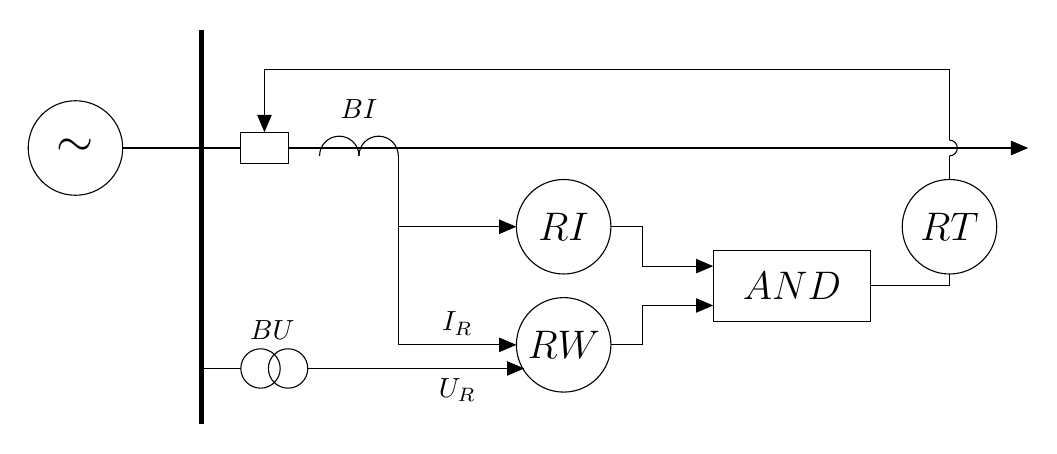
\begin{tikzpicture}[>=triangle 45]
		\draw (-.1,0) circle (.6)  node{\LARGE{$\mathbf{\sim}$}};
		\draw (0.5, 0) -- (1.5,0);
		\draw[ultra thick] (1.5,1.5) -- (1.5, -3.5);
		\draw (1.5,0) -- (2,0); \draw (2,0.2) rectangle (2.6,-0.2); \draw[->] (2.6,0) -- (12,0);
		\draw (3.5,-0.1) arc (0:180:0.25); \draw (4,-0.1) arc (0:180:0.25); \draw (3.5,0.25) node[above]{$BI$}; \draw (4,-0.1) -- (4,-1); \draw[->] (4,-1) -- (5.5,-1); \draw (6.1,-1) circle (.6)  node{\Large{$RI$}}; \draw (6.7,-1) -- (7.1,-1) -- (7.1,-1.5); \draw[->] (7.1,-1.5) -- (8,-1.5);
		\draw (4,-1) -- (4,-2.5); \draw[->] (4,-2.5) -- (5.5,-2.5);\draw (6.1,-2.5) circle (.6)  node{\Large{$RW$}};  \draw (6.7,-2.5) -- (7.1,-2.5) -- (7.1,-2); \draw[->] (7.1,-2) -- (8,-2);  \draw (4.75,-2.5) node[above] {$I_R$};
		\draw (8,-1.3) rectangle (10, -2.2); \draw (9,-1.75) node{\Large{$AND$}}; \draw (10,-1.75) -- (11,-1.75) -- (11,-1.6); \draw (11,-1) circle (0.6) node{\Large{$RT$}} ; \draw (11,-0.4) -- (11,-0.1); \draw (11,-0.1) arc (-90:90:0.1); \draw (11,0.1) -- (11,1) -- (2.3,1); \draw[->] (2.3,1) -- (2.3,0.2);
		\draw (1.5,-2.8) -- (2,-2.8); \draw (2.25,-2.8) circle (.25); \draw (2.6,-2.8) circle (.25); \draw (2.4, -2.55) node[above] {$BU$}; \draw[->] (2.85,-2.8) -- (5.6,-2.8); \draw (4.75, -2.8) node[below]{$U_R$};
	\end{tikzpicture}
\end{document} 